\newpage

\section{Objetivo}
Revisar o uso de aplificadores operacionais, que são muito utilizados na instrumentação eletrônica.

\section{Introdução}

\subsection{Experimento 1}
Nesse experimento foi utilizado um diodo zenner como tensão de referência para a leitura de uma resistência.

\begin{figure}[H]
\begin{center}
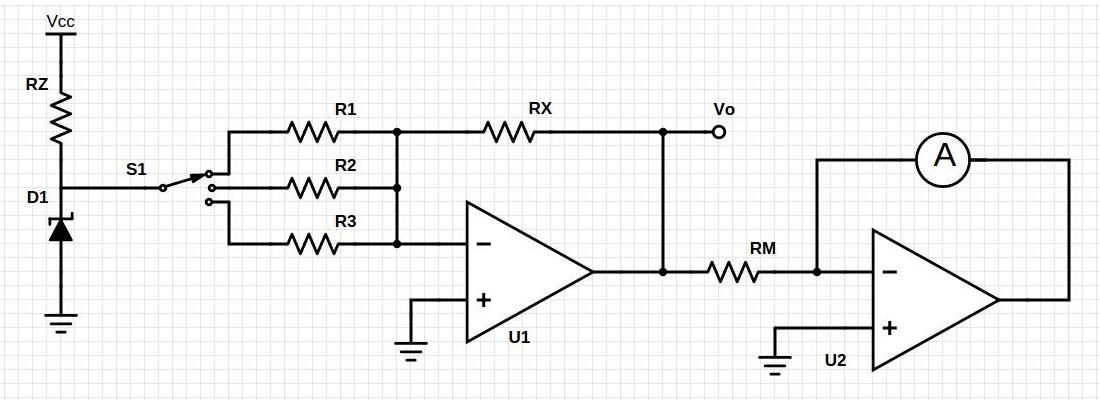
\includegraphics[scale=.25]{Imagens/cir1.jpg}
\caption{Circuito com três escalas de resistência.}
\label{cir1}
\end{center}
\end{figure}

\begin{itemize}
 \item Calcular o valor de Rz.
 \item Calcular o valor de R1, R2 e R3 de modo que fiquem três escalas distintas para a medição da resistência.
 \item Calcular o valor de Rm para limitar a corrente de acordo com a escala do amperímetro.
 \item Montar o circuito da figura 1 e utilizar 2 valores de resistência para cada escala. Medir a corrente no amperímetro e anotar os valores obtidos.
 \end{itemize} 
 
 \subsection{Experimento 2}
Neste experimento foi projetado um circuito amplificador com ganho controlado digitalmente. 
 
\begin{figure}[H]
\begin{center}
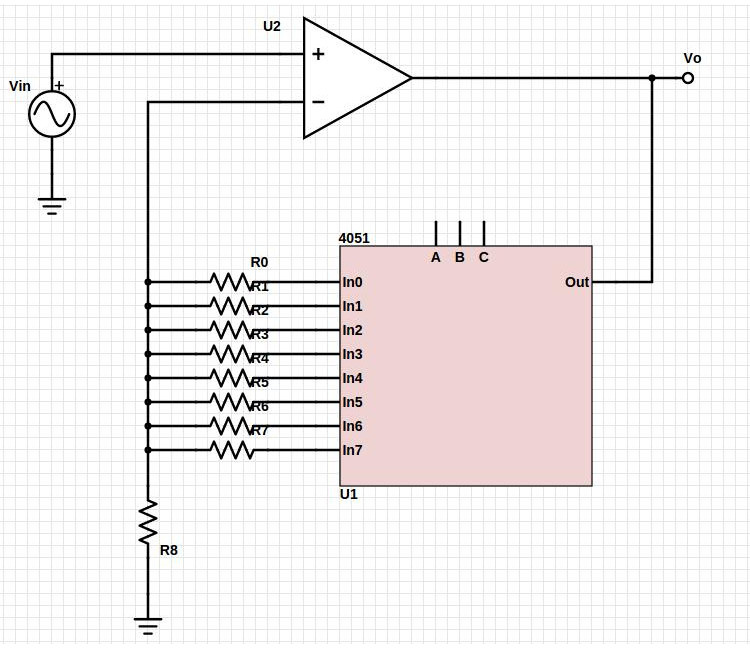
\includegraphics[scale=.3]{Imagens/cir2.jpg}
\caption{Amplificador com ganho variável.}
\label{cir2}
\end{center}
\end{figure}

\begin{itemize}
 \item Definir o valor dos resistores para 8 ganhos diferentes.
 \item Montar o circuito da \ref{cir2} e aplicar um sinal senoidal na entrada.
 \item Analizar o ganho do circuito.
 \end{itemize} 